\subsection{高斯判别分析：LDA及其扩展}
\label{sec:classification-gda}

朴素贝叶斯只保存每维的均值与方差，相当于把类内协方差矩阵的非对角元素设为零。这个约束可能丢失决定类别的信息。设两类二维高斯数据的均值都为零，每一维的方差都为$1$，但类1中两个测量值通常一起增减，类2中则通常一个增大、另一个减小。两类的单维分布完全相同，高斯NB只能依据先验比例判类；联合分布却分别沿两个不同方向伸展。

\term{高斯判别分析}（Gaussian discriminant analysis, GDA）为每类估计多元高斯分布，用协方差保留这种共同变化。在上述例子中，两类不同的非对角协方差进入判别得分，就能利用单维统计量遗漏的方向信息。共享协方差形式对应\term{线性判别分析}（linear discriminant analysis, LDA），各类分别估计协方差则对应QDA。完整协方差同时增加了参数量；样本较少时，收缩估计仍可能比完全放开的估计更合适。

第\ref{sec:clustering-gmm}节的高斯混合模型同样估计高斯成分及其权重，但成分归属是潜变量，通常用\term{期望最大化}（expectation-maximization, EM）交替计算成分归属的后验概率并更新分布参数；两步计算的分类实例见第\ref{sec:classification-self-training-soft-em}节。GDA中的类别标签已经观测，可以直接按类分组估计。两者共享高斯密度结构，却分别服务于预设类别预测和无标签分组。

\subsubsection{模型结构}
\label{sec:classification-lda-model}

沿用训练集$D_n=\{(\bm{x}_i,y_i)\}_{i=1}^{n}$，其中$\bm{x}_i\in\mathbb{R}^{d}$、$y_i\in\{1,\ldots,C\}$。生成式LDA假设
\begin{equation}
  \label{eq:classification-lda-distribution}
  \begin{aligned}
    \mathbb{P}(y=c)&=\pi_c,\qquad \pi_c>0,\quad
      \sum_{c=1}^{C}\pi_c=1,\\
    p(\bm{x}\mid y=c)&=\mathcal{N}(\bm{x};\bm{\mu}_c,\bm{\Sigma}),
      \qquad \bm{\Sigma}\succ0 .
  \end{aligned}
\end{equation}
这里$\bm{\mu}_c\in\mathbb{R}^{d}$描述第$c$类的中心，$\bm{\Sigma}\in\mathbb{R}^{d\times d}$描述类内各方向的波动及特征之间的相关性。共享协方差允许各类具有不同中心，同时规定中心附近相同的椭球形状和朝向；协方差中的非对角元仍可表示特征相关性。

要从类别概率得到分类规则，先固定一个输入$\bm x$，把真实类别后验记为$p_c^\ast(\bm x)=\mathbb P(Y=c\mid\bm X=\bm x)$。若决定把它判为类别$c$，正确的条件概率就是$p_c^\ast(\bm x)$，相应判错的条件概率，即零一损失的条件期望，为$1-p_c^\ast(\bm x)$。要让判错的概率最小，应选后验最大的那个类别；后验并列时，从最大者中按最小类别索引选一个，条件错误率仍相同。这样的逐输入最优规则称为\term{贝叶斯分类器}（Bayes classifier），也称贝叶斯分类规则。它的意义不是一个可以直接训练的模型（真实后验未知），而是一切分类器在理论上能达到的最好水平。

再按输入分布平均各处的最小条件错误率，就得到\term{贝叶斯风险}（Bayes risk）：
\begin{equation}
  \begin{aligned}
    f^\ast(\bm x)&=\argmax_{1\leq c\leq C}p_c^\ast(\bm x),\\
    R^\ast&=\mathbb E_{\bm X}
       \left[1-\max_{1\leq c\leq C}p_c^\ast(\bm X)\right].
  \end{aligned}
  \label{eq:classification-bayes-rule-risk}
\end{equation}
它是在全部可测分类规则中能够达到的最小零一风险，取决于输入与标签的真实共同分布，不要求使用某个特定的估计模型。真实后验通常未知，因此这个规则首先提供一个比较基准；LDA再用所设定的生成分布计算并估计后验，实际误差还取决于这些分布假设与参数估计是否合适。

在零一损失下，应选择后验概率最大的类别。对本节的生成模型，贝叶斯公式的分母是所有类别共有的输入密度，所以比较后验只需比较$\pi_c p(\bm x\mid y=c)$。取对数并展开高斯密度，有
\begin{equation}
  \label{eq:classification-lda-score}
  \begin{aligned}
    \log\{\pi_c p(\bm{x}\mid y=c)\}
      &=a(\bm{x})+\delta_c(\bm{x}),\\
    \delta_c(\bm{x})
      &=\bm{x}^{\top}\bm{\Sigma}^{-1}\bm{\mu}_c\\
      &\quad-\frac12\bm{\mu}_c^{\top}\bm{\Sigma}^{-1}\bm{\mu}_c
        +\log\pi_c .
  \end{aligned}
\end{equation}
其中$a(\bm{x})$收集了$-\bm{x}^{\top}\bm{\Sigma}^{-1}\bm{x}/2$、对数行列式和高斯归一化常数，均与类别无关。正是共享协方差使二次项在类别比较时抵消，留下关于$\bm{x}$的仿射函数。任意两类得分相等的位置通常为超平面；多分类的各类别区域由这些两两比较共同确定。

训练后把估计参数代入$\delta_c$，得到$\hat{\delta}_c$。预测规则及相应的模型后验为
\begin{equation}
  \label{eq:classification-lda-prediction}
  \begin{aligned}
    \hat f_{\mathrm{LDA}}(\bm{x})
      &=\argmax_{c\in\{1,\ldots,C\}}\hat{\delta}_c(\bm{x}),\\
    \hat p_c(\bm{x})
      &=\frac{\exp\{\hat{\delta}_c(\bm{x})\}}
        {\sum_{j=1}^{C}\exp\{\hat{\delta}_j(\bm{x})\}} .
  \end{aligned}
\end{equation}
本节对$\argmax$的平局统一选择索引最小的类别。共享协方差也限定了LDA能利用的类别差异。例如，设两类中心都在原点，一类的测量值集中在中心附近，另一类的测量值分散得更开。此时“离中心有多远”包含类别信息，但LDA中两类相同的均值使与输入有关的得分项完全相消，分类只能依据先验比例。若两类先验还相等，按真实均值形成的这组得分处处平局，固定类别的预测错误率为$1/2$。这说明共享协方差会舍弃类别之间的尺度差异。

GDA的一般模型不要求共享协方差。对第$c$类，参数是$\pi_c$、$\bm{\mu}_c\in\mathbb{R}^{d}$及对称正定的$\bm{\Sigma}_c\in\mathbb{R}^{d\times d}$：
\begin{equation}
  \label{eq:classification-gda-density}
  \begin{aligned}
    p(\bm{x}\mid y=c)
      &=\frac{\exp[-\Delta_c(\bm{x})/2]}
        {(2\pi)^{d/2}|\bm{\Sigma}_c|^{1/2}},\\
    \Delta_c(\bm{x})
      &=(\bm{x}-\bm{\mu}_c)^{\top}
        \bm{\Sigma}_c^{-1}(\bm{x}-\bm{\mu}_c).
  \end{aligned}
\end{equation}
这里的二次型$\Delta_c$按类内变化尺度衡量输入偏离均值的程度；行列式项补偿分布体积，在不同协方差的类别比较中同样参与得分。贝叶斯后验仍为$\pi_cp(\bm{x}\mid y=c)/\sum_r\pi_rp(\bm{x}\mid y=r)$。这一模型不要求各特征独立，但要求整类分布可由单个多元高斯刻画；完整协方差保留全部二阶关系，单个高斯成分仍限制了非线性依赖和多峰结构的表达。

\subsubsection{参数学习}
\label{sec:classification-lda-learning}

\paragraph{生成分布的最大似然估计}
有标签样本已经给出了每个观测所属的高斯分量，因此这里不需要推断类别归属。令$n_c=\sum_{i=1}^{n}\mathbb{1}\{y_i=c\}$，暂设各类都有样本。忽略与参数无关的常数，对数似然为
\begin{equation}
  \label{eq:classification-lda-likelihood}
  \begin{aligned}
    \ell
      &=\sum_{c=1}^{C}n_c\log\pi_c
        -\frac n2\log\det\bm{\Sigma}\\
      &\quad-\frac12\sum_{c=1}^{C}\sum_{i:y_i=c}
        (\bm{x}_i-\bm{\mu}_c)^{\top}
        \bm{\Sigma}^{-1}(\bm{x}_i-\bm{\mu}_c).
  \end{aligned}
\end{equation}
对先验加入约束$\sum_c\pi_c=1$，拉格朗日驻点给出$n_c/\pi_c$为同一常数；归一化后该常数为$n$。对$\bm{\mu}_c$求导，则有$\bm{\Sigma}^{-1}\sum_{i:y_i=c}(\bm{x}_i-\bm{\mu}_c)=\bm{0}$。由此得到
\begin{equation}
  \label{eq:classification-lda-mean-prior}
  \hat\pi_c=\frac{n_c}{n},\qquad
  \hat{\bm{\mu}}_c=\frac1{n_c}\sum_{i:y_i=c}\bm{x}_i .
\end{equation}
这两个估计分别是类别出现频率和该类的样本均值。

把均值代回似然，定义\term{类内散度矩阵}（within-class scatter matrix）
\begin{equation}
  \label{eq:classification-lda-within}
  \bm{S}_{\mathrm{W}}
    =\sum_{c=1}^{C}\sum_{i:y_i=c}
      (\bm{x}_i-\hat{\bm{\mu}}_c)
      (\bm{x}_i-\hat{\bm{\mu}}_c)^{\top}.
\end{equation}
它累加每个样本相对于本类中心的偏离。用精度矩阵$\bm{\Omega}=\bm{\Sigma}^{-1}$改写剩余目标，得到$n\log\det\bm{\Omega}/2-\operatorname{tr}(\bm{\Omega}\bm{S}_{\mathrm{W}})/2$。其驻点满足$n\bm{\Omega}^{-1}=\bm{S}_{\mathrm{W}}$，故当$\bm{S}_{\mathrm{W}}\succ0$时，
\begin{equation}
  \label{eq:classification-lda-covariance}
  \hat{\bm{\Sigma}}=\frac1n\bm{S}_{\mathrm{W}} .
\end{equation}
对$\bm{\Omega}$的目标是严格凹的，因此该驻点给出最大似然解。

式~\eqref{eq:classification-lda-covariance}的分母是$n$，不是$n-C$。这种合并各类类内变动的估计称为\term{合并协方差}（pooled covariance），其无偏形式为
\[
  \hat{\bm{\Sigma}}_{\mathrm{U}}
    =\frac{\bm{S}_{\mathrm{W}}}{n-C},\qquad n>C .
\]
在共享协方差假设下，给定各类样本数，有$\mathbb{E}[\bm{S}_{\mathrm{W}}\mid y_1,\ldots,y_n]=(n-C)\bm{\Sigma}$，因为估计每个类中心各消耗一个自由度。最大似然与无偏估计是不同准则；两种估计渐近相同，但有限样本下有所区别。特别是先验不等时，整体缩放协方差会改变几何得分相对于$\log\hat\pi_c$的权重，预测边界未必相同。

闭式估计把训练归结为统计量累计和线性代数运算。稠密数据的类内散度累计需要$O(nd^2)$运算，矩阵分解需要$O(d^3)$运算。实现时分解一次$\hat{\bm{\Sigma}}$，再解$C$个线性方程组$\hat{\bm{\Sigma}}\bm{a}_c=\hat{\bm{\mu}}_c$；预存$\bm{a}_c$与常数项后，每个样本的预测成本为$O(Cd)$。这些计算要求协方差可逆。$\bm{S}_{\mathrm{W}}$奇异时，正定参数域内的最大似然解不存在，需用降维或正则化重新规定估计问题。类特有协方差采用MLE分母$n_c$；若改用$n_c-1$，得到的是无偏估计。当某类散度奇异时，沿未被样本覆盖的方向收缩方差会使似然不断增大，正定参数域内便没有有限MLE。此时必须先规定共享、对角或收缩等估计方案，不能把奇异样本散度直接作为普通高斯协方差。

\subsubsection{与Fisher投影的对应}
\label{sec:classification-gda-fisher-relation}

生成模型之外，第\ref{sec:classification-fisher}节的Fisher准则直接比较投影后的类间分离与类内波动。二分类时令$\bm{h}=\hat{\bm{\mu}}_1-\hat{\bm{\mu}}_2\ne\bm{0}$，由总均值的定义可得
\[
  \bm{S}_{\mathrm{B}}=\frac{n_1n_2}{n}\bm{h}\bm{h}^{\top},
  \qquad
  \bm{w}_{\mathrm{F}}\propto\bm{S}_{\mathrm{W}}^{-1}\bm{h}.
\]
生成式LDA的法向量则为$\bm{w}_{\mathrm{G}}=\hat{\bm{\Sigma}}^{-1}\bm{h}=n\bm{S}_{\mathrm{W}}^{-1}\bm{h}$，两者方向相同。但完整的生成式分类规则还比较两类得分差的正负，其中含先验项$\log(\hat\pi_1/\hat\pi_2)$：
\begin{equation}
  \label{eq:classification-lda-binary-threshold}
  \hat\delta_1(\bm{x})-\hat\delta_2(\bm{x})
    =\bm{w}_{\mathrm{G}}^{\top}
      \left(\bm{x}-\frac{\hat{\bm{\mu}}_1+\hat{\bm{\mu}}_2}{2}\right)
      +\log\frac{\hat\pi_1}{\hat\pi_2}.
\end{equation}
Fisher准则本身只给方向，不给类先验、后验概率或这一阈值。两类均值相同时，均值散度准则没有正特征值方向，而生成模型仍可按先验选择类别。因此Fisher投影可用于非高斯数据，而贝叶斯最优性的证明还需要正确指定的高斯生成模型。

\subsubsection{支持不同类内尺度与方向：QDA}
\label{sec:classification-lda-covariance-extensions}

如果不同类别的类内变化方向和尺度明显不同，共享协方差就会限制LDA的表达能力。\term{二次判别分析}（quadratic discriminant analysis, QDA）保留类条件高斯假设，却为每个类别估计独立的协方差矩阵$\hat{\bm{\Sigma}}_c$\scite{hastie2009}。先假设各类协方差估计均正定，删去各类共同的常数项后，其判别得分为
\begin{equation}
  \begin{aligned}
    \delta_c(\bm{x})
      ={}&\log\hat{\pi}_c-\frac12\log\det\hat{\bm{\Sigma}}_c\\
        &-\frac12(\bm{x}-\hat{\bm{\mu}}_c)^\top
          \hat{\bm{\Sigma}}_c^{-1}(\bm{x}-\hat{\bm{\mu}}_c).
  \end{aligned}
  \label{eq:classification-qda-score}
\end{equation}
展开马氏项，得分中关于$\bm{x}$的二次部分为$-\tfrac12\bm{x}^{\top}\hat{\bm{\Sigma}}_c^{-1}\bm{x}$，线性部分为$\bm{x}^{\top}\hat{\bm{\Sigma}}_c^{-1}\hat{\bm{\mu}}_c$。任意两类得分之差因此含有关于$\bm{x}$的二次项，边界一般是二次曲面。当两类协方差相同时，二次项$\bm{x}^{\top}\hat{\bm{\Sigma}}^{-1}\bm{x}$在相减时完全相同而抵消，只剩线性项$\bm{x}^{\top}\hat{\bm{\Sigma}}^{-1}(\hat{\bm{\mu}}_c-\hat{\bm{\mu}}_{c'})$，边界又退化为直线/超平面，即LDA。增加自由度也增加了估计负担：共享协方差模型需要$O(d^2+Cd)$个参数，QDA则需要$O(Cd^2)$个参数；每一类只有少量样本时，独立协方差容易不稳定甚至奇异。参数学习仍使用有标签的最大似然：类先验和均值沿用式\eqref{eq:classification-lda-mean-prior}，第$c$类协方差改为
\[
  \hat{\bm\Sigma}_c=\frac1{n_c}\sum_{i:y_i=c}
    (\bm x_i-\hat{\bm\mu}_c)(\bm x_i-\hat{\bm\mu}_c)^\top.
\]
把这些估计代入式\eqref{eq:classification-qda-score}，取最高得分类别，就完成训练到预测的连接。若某类协方差奇异，应先采用下文的收缩等处理，不能直接把它代入普通高斯密度。

图\ref{fig:classification-gaussian-boundaries}在同一个二维教学例子中比较两种协方差设定。两图都取$\pi_1=\pi_2=1/2$、$\bm{\mu}_1=(-1,0)^{\top}$、$\bm{\mu}_2=(1,0)^{\top}$，坐标为无量纲特征。左图共享$\bm{\Sigma}_1=\bm{\Sigma}_2=\bm{I}_2$；右图只将第2类改为$\bm{\Sigma}_2=\operatorname{diag}(1,4)$。按式\eqref{eq:classification-qda-score}计算，得分差分别为
\begin{equation}
  \label{eq:classification-gda-boundary-example}
  \begin{aligned}
    g_2-g_1&=2x_1
      &&\text{（共享协方差）},\\
    g_2-g_1&=2x_1+\frac38x_2^2-\log2
      &&\text{（类特有协方差）}.
  \end{aligned}
\end{equation}
令得分差为零，得到直线$x_1=0$和抛物线$x_1=\frac12\log2-\frac{3}{16}x_2^2$。在两种设定中，边界右侧的$g_2$都更大，预测第2类。右图中，第2类沿$x_2$方向更分散：在$x_2=0$附近，行列式项降低了它的密度峰值，边界向右移到$x_1\approx0.347$；随着$|x_2|$增大，第2类较慢衰减的密度又使其预测区域向左延伸。只看均值之间的距离，会漏掉方差尺度和密度归一化对判决的共同影响。
\begin{figure*}[htbp]
  \centering
  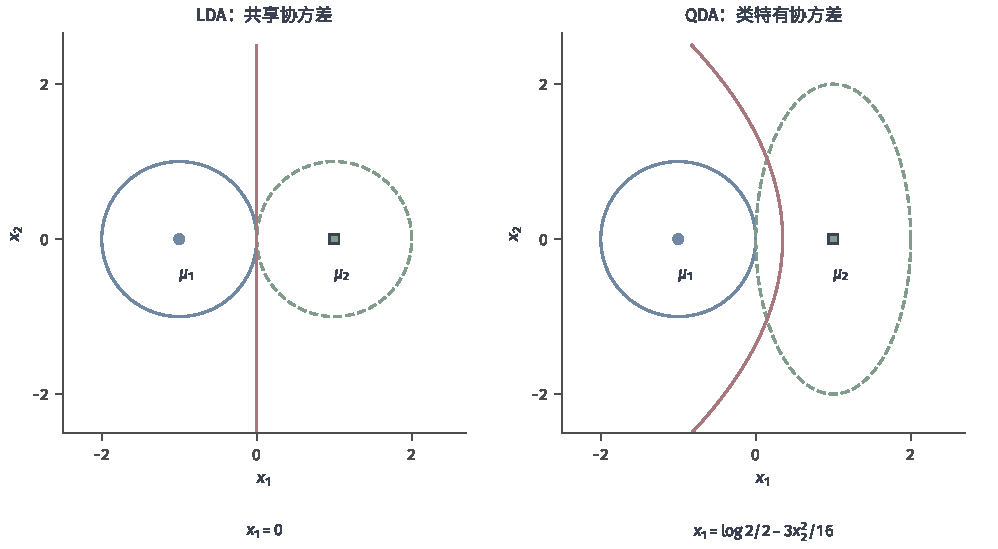
\includegraphics[width=159.059mm]{figures/07-classic-models/00-shared/matplotlib/classification-gaussian-boundaries/figure.pdf}
  \caption{两图均取$\pi_1=\pi_2=1/2$、$\bm{\mu}_1=(-1,0)^{\top}$、$\bm{\mu}_2=(1,0)^{\top}$和$\bm{\Sigma}_1=\bm{I}_2$，仅第2类协方差变化。蓝色圆点和绿色方点为均值，蓝色实线与绿色虚线分别为$\Delta_1=1$和$\Delta_2=1$的等密度轮廓；不同类的这些轮廓不保证密度值相同。红色粗线按$g_1=g_2$的解析式绘制，底部公式分别给出LDA的线性边界与QDA的二次边界。参数均为教学构造，不是采样或拟合结果。}
  \label{fig:classification-gaussian-boundaries}
\end{figure*}

完整协方差每类需要$d(d+1)/2$个自由参数。类内散布矩阵的秩至多为$n_c-1$，因而$n_c\leq d$时必然奇异，不能直接代入普通高斯密度；$n_c>d$也不保证估计准确或条件良好。共享估计的秩至多为$n-C$。在维数较大或类别样本少时，可以共享、取对角，或采用下面的RDA收缩估计。

\subsubsection{缓解小样本协方差不稳定：RDA}
\label{sec:classification-gda-rda}

QDA放开了各类的形状，但少数类可能没有足够样本估计完整协方差。例如，一个类别只有10个样本，中心化后的样本协方差秩至多为9；若输入有20维，这个估计便无法求逆。完全改用LDA又会舍弃类间真实的尺度或方向差异。可以在两者之间折中，让各类借用一部分合并统计量。\term{正则化判别分析}（regularized discriminant analysis, RDA）通过收缩协方差控制这种取舍。Friedman的原始方法包含两个调节方向：将类内协方差向合并协方差收缩，再向球形协方差收缩\scite{friedman1989rda}。

这里两种协方差统计量都使用最大似然形式的归一化。记$n_c>0$为第$c$类样本数，并令
\[
  \begin{aligned}
    \hat{\bm{\Sigma}}_c
      &=\frac{1}{n_c}\sum_{i:y_i=c}
        (\bm{x}_i-\hat{\bm{\mu}}_c)
        (\bm{x}_i-\hat{\bm{\mu}}_c)^{\top},\\
    \hat{\bm{\Sigma}}
      &=\frac1n\sum_{c=1}^{C}n_c\hat{\bm{\Sigma}}_c.
  \end{aligned}
\]
这些样本散度矩阵允许奇异；在收缩获得正定矩阵以前，不能把奇异统计量直接代入普通高斯密度。RDA先混合类内与合并统计量，再向球形协方差收缩，一种相应写法是
\begin{equation}
  \begin{aligned}
    \bm{A}_c(a)
      &=\frac{(1-a)n_c\hat{\bm{\Sigma}}_c+an\hat{\bm{\Sigma}}}
              {(1-a)n_c+an},\\
    \tilde{\bm{\Sigma}}_c(a,b)
      &=(1-b)\bm{A}_c(a)
        +b\,\frac{\operatorname{tr}\bm{A}_c(a)}{d}\bm{I},
        \qquad a,b\in[0,1].
  \end{aligned}
  \label{eq:classification-rda}
\end{equation}
当$b=0$时，$a=0$与$a=1$分别对应QDA与LDA的协方差统计量。增大$a$让每类更多地借用共同统计量；增大$b$则把各方向的方差拉向同一个平均值，并抑制非对角的协方差项。这不是把整份协方差按同一比例缩小。平均方差为正时，正的球形收缩权重有助于获得可逆估计。均值与先验仍按原有类统计量估计，再把收缩后的协方差代入QDA得分；两个参数应在训练集内部通过验证选择。当合并协方差和各类协方差均奇异时，可逆性还需要平均方差为正的球形收缩项或其他正则化。

收缩也改变哪些类别差异能够进入得分。$a=1,b=0$时各类共享协方差，二次项相消；$b=1$时每类协方差都为单位矩阵的一个倍数，得分可以利用半径平方，却不能独立利用各方向的方差与特征相关性。只有保留完整的类特有协方差，才能表达前面QDA中的一般二次差异。RDA是在这些限制与估计波动之间选择，不是一个可以越过QDA分布族的新模型。收缩强度越大，类形状越受限制；强度越小，越依赖每类样本估计完整协方差。应在训练数据内部选择强度，再检查独立数据上的分类误差与估计稳定性。

\subsubsection{高斯模型与直接概率模型的关系}
\label{sec:classification-gda-direct-relation}

对二分类，把式~\eqref{eq:classification-lda-score}中的两类得分相减并归一化，就得到Logistic形式的后验。因此，共享高斯假设蕴含线性对数几率，反过来却不成立；许多非高斯输入分布也能有Logistic形式的条件概率。即便两条路线的后验形式相同，用联合似然估计均值和协方差，与直接最大化条件似然（第\ref{sec:classification-logistic}节），也通常得到不同的有限样本参数。前者是生成式，先拟合输入分布；后者是判别式，只拟合条件概率。

稠密完整协方差的统计成本约为$O(nd^2)$，各类矩阵分解约为$O(Cd^3)$，存储为$O(Cd^2)$，QDA单样本得分约为$O(Cd^2)$。LDA只需分解一份协方差，并可预先算出线性权重，使单样本预测降到$O(Cd)$。实现时可用Cholesky分解求解二次型与对数行列式，无须显式构造逆矩阵。

表\ref{tab:classification-probability-comparison}汇总相同监督分类任务下生成式与判别式概率模型的主要取舍。参数量按每维分布参数有界计算，GDA的共享与类特有协方差分别列明，避免把两者的代价混在一起。
\begin{table}[htbp]
  \centering
  \small
  \begin{tabularx}{\linewidth}{@{}
    >{\RaggedRight\arraybackslash}p{0.19\linewidth}
    >{\RaggedRight\arraybackslash}X
    >{\RaggedRight\arraybackslash}X@{}}
    \toprule
    模型 & 建模与估计 & 主要取舍 \\
    \midrule
    Logistic回归／Softmax回归 &
    直接拟合条件概率；$O(Cd)$个参数，迭代优化 &
    不拟合输入分布；需检查特征表示、分离与正则化 \\
    NB &
    由先验和简化类条件模型形成后验；通常$O(Cd)$个参数 &
    计数或矩估计易累积；依赖和事件模型失配会引入偏差 \\
    共享GDA（LDA） &
    高斯类条件分布，共享协方差；$O(d^2+Cd)$个参数 &
    用共同协方差降低估计波动；只得到线性边界 \\
    类特有GDA（QDA） &
    各类独立估计协方差；$O(Cd^2)$个参数 &
    边界更灵活；对每类样本量和协方差条件更敏感 \\
    \bottomrule
  \end{tabularx}
  \caption{概率分类模型的建模对象与估计代价。所有概率输出都需单独检查校准，参数量不直接等于达到指定精度所需的样本量。}
  \label{tab:classification-probability-comparison}
\end{table}

类条件假设可以减轻小样本下的估计负担，也可能留下模型失配。Ng和Jordan对特定NB与判别式模型的研究展示了这种取舍，不能据此给全部生成式与判别式模型排序\scite{ng2001}。实际选择应固定输入表示、数据划分、误判代价和调参预算，比较分类错误、概率质量与计算成本；训练误差更小或输出取值合法，都不能单独说明概率已经可靠。
